\subsection{Overview}
CLup is an application aimed at decreasing the probability of contracting COVID-19 (diseases in general) when going shopping to a supermarket. There are two fundamental components: the main one targets customers of supermarkets while the second one is available for store managers.\newline
\subsubsection{User Interfaces}
\paragraph{End user functionalities}
Regarding the first target - customers - they will be required to register to the service the first time they use it by inserting their full name, email address, ID card, phone number and a password. The customer will also be requested to specify his physical address, or to enable the GPS, in order to allow CLup to find stores nearby; this last information can be changed anytime the user needs. If the customer is not willing to register or share his address, the service will not be available.
\begin{figure}[h!]
	\centering
	\begin{subfigure}[b]{0.3\textwidth}
		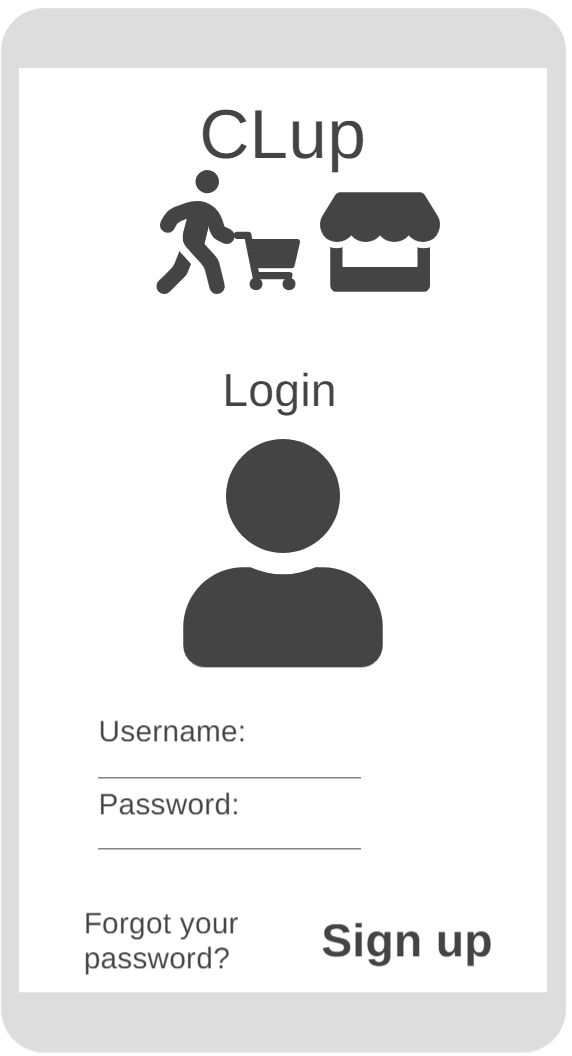
\includegraphics[width=\linewidth]{../Diagrams/WireframesCLup/Login.png}
		\caption{Login screen}
		\label{fig:WfLogin}
	\end{subfigure}
	\hfill
	\begin{subfigure}[b]{0.3\textwidth}
		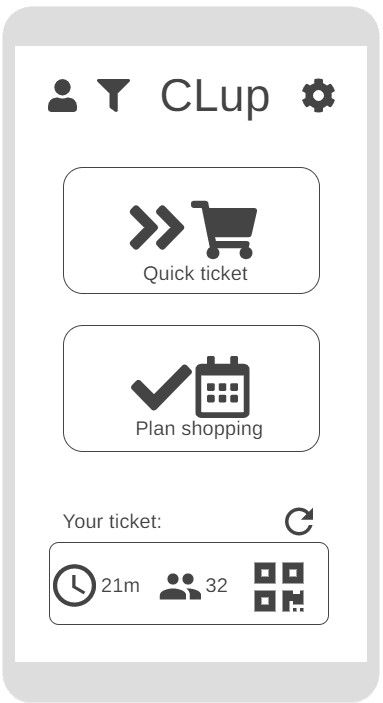
\includegraphics[width=\linewidth]{../Diagrams/WireframesCLup/MainScreen.png}
		\caption{Main screen}
		\label{fig:WfMain}
	\end{subfigure}
	\caption{App startup}
	\label{fig:Wireframes}
\end{figure}
Once the setup is done, customers will be able to access the homepage of the application, where they can tap on a “Virtually queue” button that will allow them to see a list of stores inside a specified range from their current location: for each store a distance in kilometers from the user position will be outlined, as well as the number of people inside the store and its maximum capacity; whenever a store is full, the current number of people in line and an \textit{EWT} are displayed.\newline  
It is also possible to visualize stores on a map and, by tapping on one of them, to see the same information displayed in the list. Now, if the user chooses to reserve a spot in the line, the application will open a confirm dialog specifying EWT and the expiration of the ticket. If the user refuses nothing happens, if he accepts instead CLup will process the request, show his ticket and the real time evolution of the line; the ticket is also visible from the home screen. The process is shown in Figure ~\ref{fig:VirtuallyQ}.\\
\begin{figure}[h!]
	\centering
	\begin{subfigure}[b]{0.3\textwidth}
		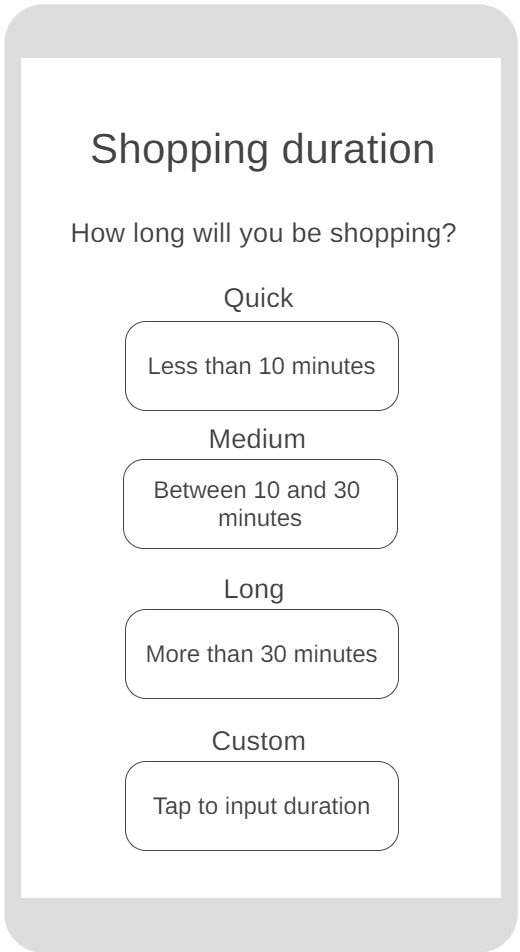
\includegraphics[width=\linewidth]{../Diagrams/WireframesCLup/ShoppingTime.png}
		\caption{Shopping time}
		\label{fig:WfShoppingTime}
	\end{subfigure}
	\hfill
	\begin{subfigure}[b]{0.3\textwidth}
		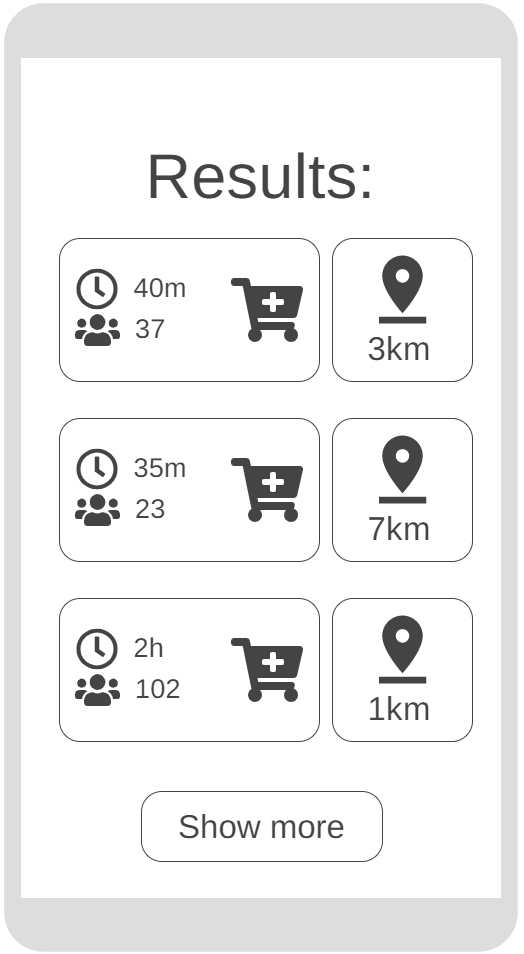
\includegraphics[width=\linewidth]{../Diagrams/WireframesCLup/QuickTicket.png}
		\caption{Store list}
		\label{fig:WfStoreList}
	\end{subfigure}
	\hfill
	\begin{subfigure}[b]{0.3\textwidth}
		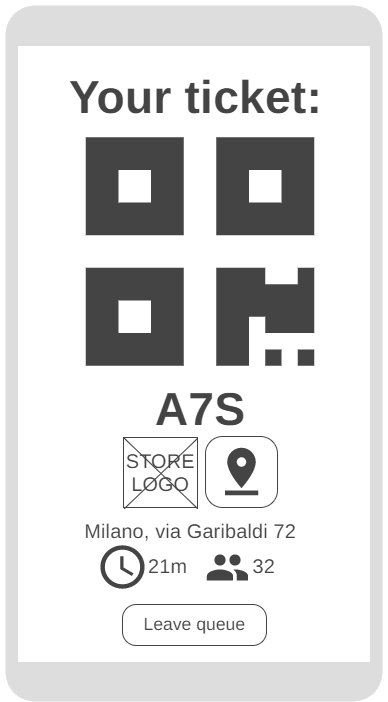
\includegraphics[width=\linewidth]{../Diagrams/WireframesCLup/Ticket.png}
		\caption{Your ticket}
		\label{fig:WfTicket}
	\end{subfigure}
	\caption{Quick ticket procedure}
	\label{fig:Wireframes}
\end{figure}
The tickets consist of a QR code and an easy to remember alphanumeric code alternative to enter the store. There will also be monitors that show the numbers allowed to enter and, eventually, delays.\newline
The distance range in which CLup will look for supermarkets is specified by the user through the filter button in the homepage, this button will in fact open the filter screen in which, among other parameters, a sliding bar controls the distance and a drop-down list allows the user to filter the chains of supermarkets.\newline
\begin{figure}[h!]
	\centering
	\begin{subfigure}[b]{0.3\textwidth}
		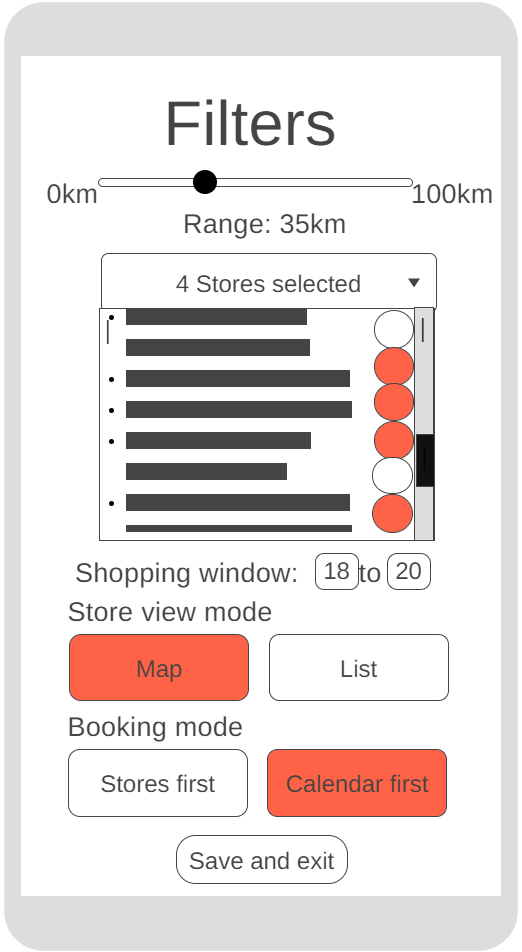
\includegraphics[width=\linewidth]{../Diagrams/WireframesCLup/Filters.png}
		\caption{Filters screen}
		\label{fig:WfFilters}
	\end{subfigure}
	\caption{Filters}
	\label{fig:Wireframes}
\end{figure}
Another important feature is the possibility to book an entrance later in the day or in another day. The user can specify from the filters whether he prefers to choose the day or the store first and he can set the time range in which he wants to book. 
There is a dedicated button in the app’s main screen that redirects the user to either the list/map of supermarkets or the calendar, and once the user chooses he will be respectively shown the calendar or the list/map, this time with colours to indicate the average crowdedness of stores/days given the set time range.
When the user chooses the day and supermarket combination, a timetable spanning the chosen time range is shown, divided in 15 minutes time slots each one having again a colour to indicate the crowdedness. The user will be able to check his reservation on the home page and near the entrance time he will be provided an actual ticket.\\
\begin{figure}[h!]
	\centering
	\begin{subfigure}[b]{0.3\textwidth}
		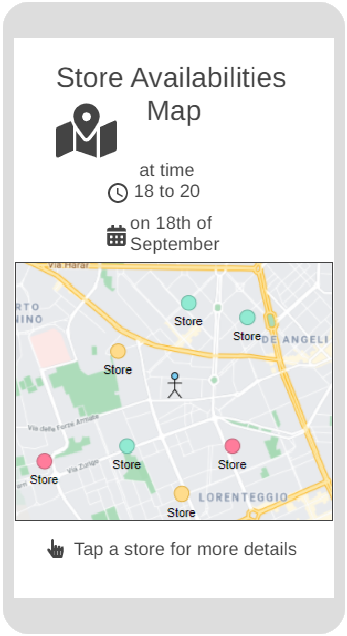
\includegraphics[width=\linewidth]{../Diagrams/WireframesCLup/StoreMap.png}
		\caption{Map screen}
		\label{fig:WfStoreMap}
	\end{subfigure}
	\hfill
	\begin{subfigure}[b]{0.3\textwidth}
		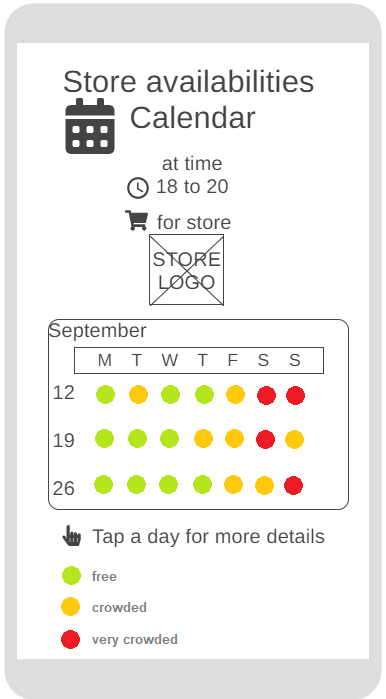
\includegraphics[width=\linewidth]{../Diagrams/WireframesCLup/Calendar.png}
		\caption{Calendar screen}
		\label{fig:WfCalendar}
	\end{subfigure}
	\hfill
	\begin{subfigure}[b]{0.3\textwidth}
		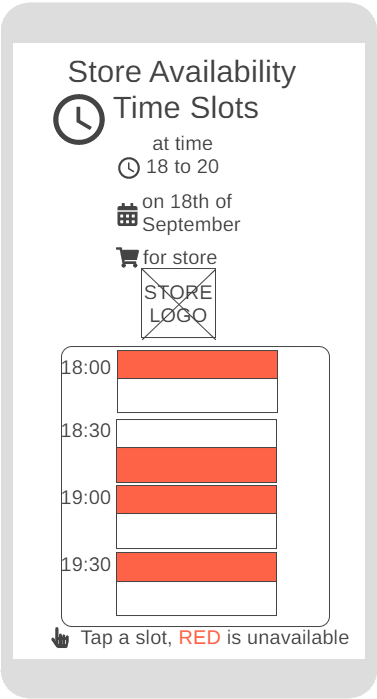
\includegraphics[width=\linewidth]{../Diagrams/WireframesCLup/TimeSlots.png}
		\caption{Time slot choice}
		\label{fig:WfTimeSlots}
	\end{subfigure}
	\caption{Booking procedure}
	\label{fig:Wireframes}
\end{figure}
The access at the supermarket is restricted by turnstiles with QR code readers, a staff member is expected to verify that nobody waits his turn in front of the entrance, jumps the turnstile or does anything irresponsible.
\begin{figure}[h!]
	\centering
	\begin{subfigure}[b]{0.3\textwidth}
		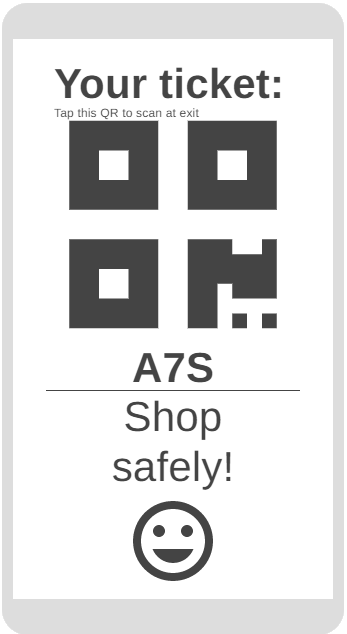
\includegraphics[width=\linewidth]{../Diagrams/WireframesCLup/Exit.png}
		\caption{Shopping screen}
		\label{fig:WfExit}
	\end{subfigure}
	\hfill
	\begin{subfigure}[b]{0.3\textwidth}
		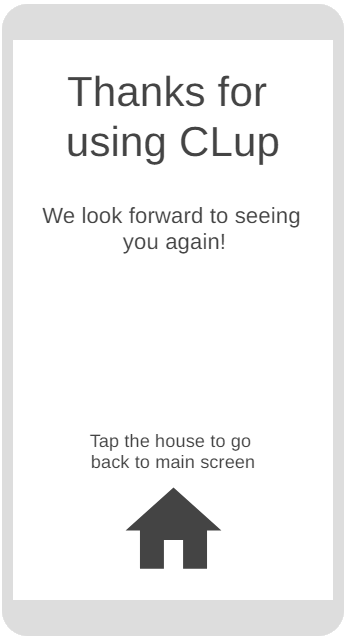
\includegraphics[width=\linewidth]{../Diagrams/WireframesCLup/FinishNoRating.png}
		\caption{Exit screen}
		\label{fig:WfFinishNoRating}
	\end{subfigure}
	\caption{Shop and exit}
	\label{fig:Wireframes}
\end{figure}
Customers who, for any reason, do not use the app will still be able to queue in CLup supermarkets by obtaining a printed ticket from a physical totem located near such stores; the functioning of the application will be similar to the “Quick ticket” app function with the difference that the user can only obtain a ticket by using a totem. \\
\begin{figure}[h!]
	\centering
	\begin{subfigure}[b]{0.3\textwidth}
		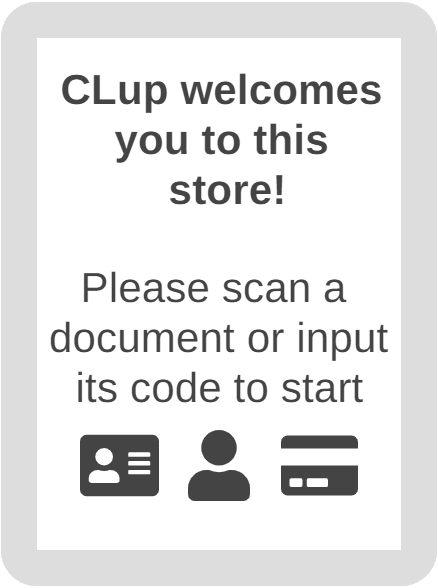
\includegraphics[width=\linewidth]{../Diagrams/WireframesCLup/TotemStart.png}
		\caption{Totem welcome screen}
		\label{fig:WfTotemStart}
	\end{subfigure}
	\hfill
	\begin{subfigure}[b]{0.3\textwidth}
		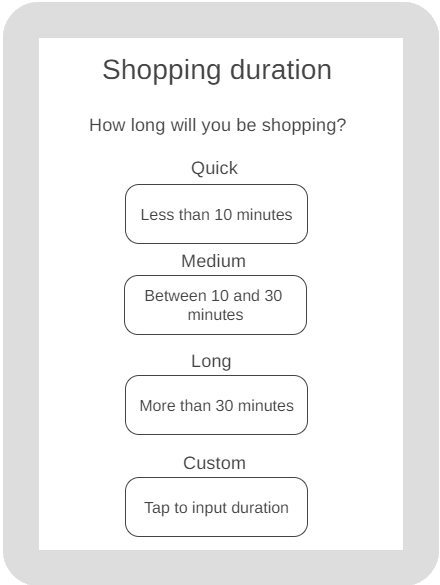
\includegraphics[width=\linewidth]{../Diagrams/WireframesCLup/TotemTime.png}
		\caption{Totem shopping time input}
		\label{fig:WfTotemTime}
	\end{subfigure}
	\hfill
	\begin{subfigure}[b]{0.3\textwidth}
		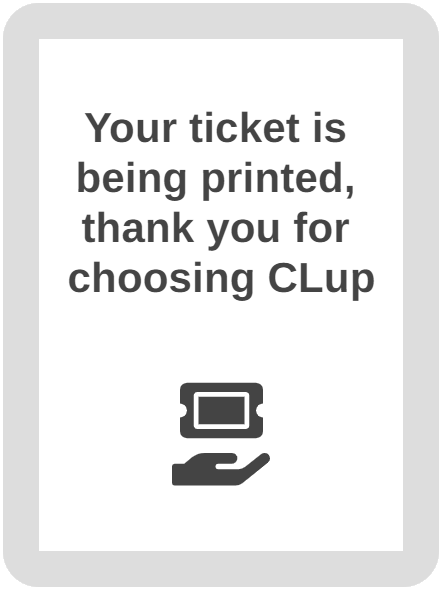
\includegraphics[width=\linewidth]{../Diagrams/WireframesCLup/TotemPrint.png}
		\caption{Totem print screen}
		\label{fig:WfTotemPrint}
	\end{subfigure}
	\caption{Totem ticket procedure}
	\label{fig:Wireframes}
\end{figure}

\paragraph{Internal use functionalities}
Another component of CLup targets store managers: when the store decides to join the CLup network, ad-hoc credentials to access the web app will be given. Special staff-only functions will then be achieved by the use of a web application, accessible via internal-use terminals.
\begin{figure}[h!]
	\centering
	\begin{subfigure}[b]{0.3\textwidth}
		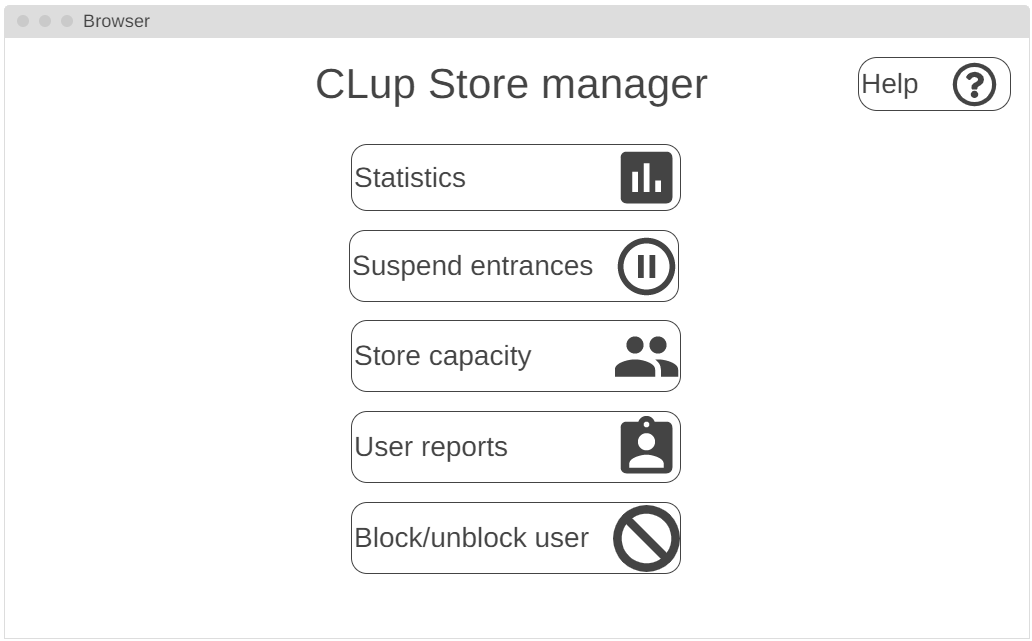
\includegraphics[width=\linewidth]{../Diagrams/WireframesCLup/ManagerMain.png}
		\caption{Manager login}
		\label{fig:WfManagerMain}
	\end{subfigure}
	\hfill
	\begin{subfigure}[b]{0.3\textwidth}
		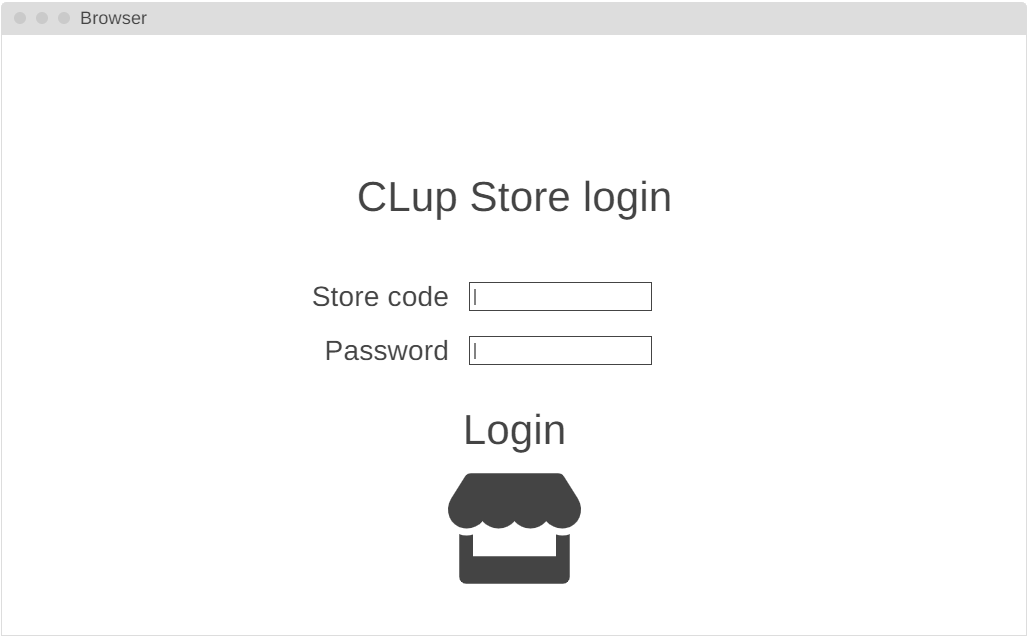
\includegraphics[width=\linewidth]{../Diagrams/WireframesCLup/ManagerLogin.png}
		\caption{Manager main screen}
		\label{fig:WfManagerLogin}
	\end{subfigure}
	\hfill
	\begin{subfigure}[b]{0.3\textwidth}
		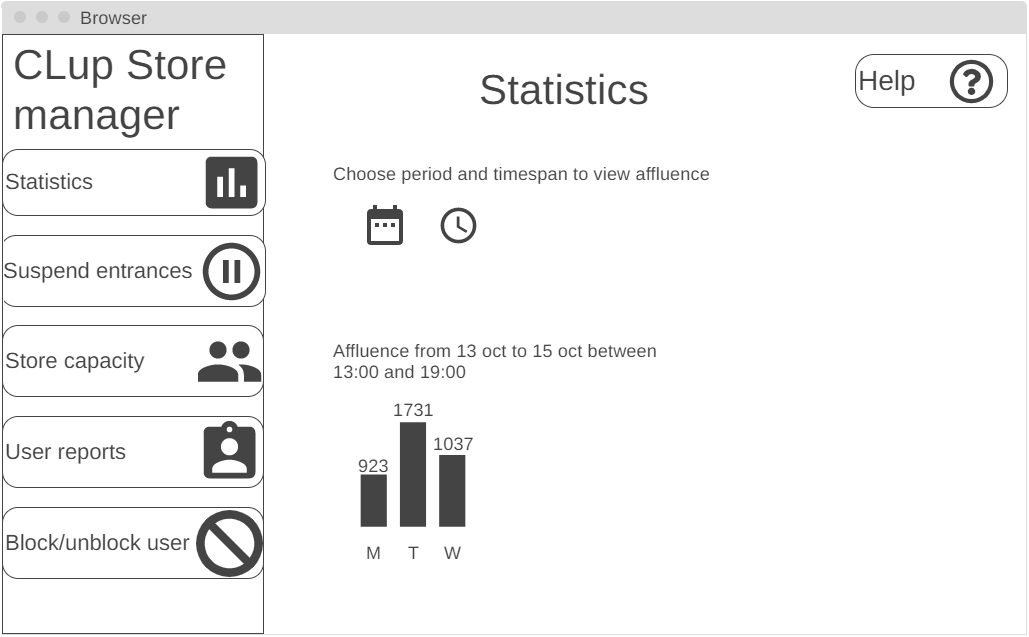
\includegraphics[width=\linewidth]{../Diagrams/WireframesCLup/ManagerStatistics.png}
		\caption{Manager statistics screen}
		\label{fig:WfManagerStatistics}
	\end{subfigure}
	\caption{Store manager web app}
	\label{fig:Wireframes}
\end{figure}
